% !TeX spellcheck = hu_HU
% !TeX encoding = UTF-8
% !TeX program = xelatex
% TODO Change language to en_GB (recommended) or en_US for English documents
\documentclass[11pt,a4paper,oneside]{report}             % Single-side
%\documentclass[11pt,a4paper,twoside,openright]{report}  % Duplex

% thanks to http://tex.stackexchange.com/a/47579/71109
\usepackage{ifxetex}
\usepackage{ifluatex}
\newif\ifxetexorluatex % a new conditional starts as false
\ifnum 0\ifxetex 1\fi\ifluatex 1\fi>0
   \xetexorluatextrue
\fi

\ifxetexorluatex
  \usepackage{fontspec}
\else
  \usepackage[T1]{fontenc}
  \usepackage[utf8]{inputenc}
  \usepackage[lighttt]{lmodern}
\fi

\usepackage[english,magyar]{babel} % Alapértelmezés szerint utoljára definiált nyelv lesz aktív, de később külön beállítjuk az aktív nyelvet.

%\usepackage{cmap}
\usepackage{amsfonts,amsmath,amssymb} % Mathematical symbols.
%\usepackage[ruled,boxed,resetcount,linesnumbered]{algorithm2e} % For pseudocodes. % beware: this is not compatible with LuaLaTeX, see http://tex.stackexchange.com/questions/34814/lualatex-and-algorithm2e
\usepackage{booktabs} % For publication quality tables for LaTeX
\usepackage{graphicx}
\usepackage{multirow}

%\usepackage{fancyhdr}
%\usepackage{lastpage}

\usepackage{anysize}
%\usepackage{sectsty}
\usepackage{setspace} % For setting line spacing

\usepackage[unicode]{hyperref} % For hyperlinks in the generated document.
\usepackage{xcolor}
\usepackage{listings} % For source code snippets.

\usepackage[amsmath,thmmarks]{ntheorem} % Theorem-like environments.

\usepackage[hang]{caption}

\singlespacing

%% Saját hozzáadott packagek
\usepackage{float}
\usepackage{breqn}
\usepackage{enumerate}
%% 

\newcommand{\selecthungarian}{
	\selectlanguage{magyar}
	\setlength{\parindent}{2em}
	\setlength{\parskip}{0em}
	\frenchspacing
}

\newcommand{\selectenglish}{
	\selectlanguage{english}
	\setlength{\parindent}{0em}
	\setlength{\parskip}{0.5em}
	\nonfrenchspacing
	\renewcommand{\figureautorefname}{Figure}
	\renewcommand{\tableautorefname}{Table}
	\renewcommand{\partautorefname}{Part}
	\renewcommand{\chapterautorefname}{Chapter}
	\renewcommand{\sectionautorefname}{Section}
	\renewcommand{\subsectionautorefname}{Section}
	\renewcommand{\subsubsectionautorefname}{Section}
}






%TODO Set the main variables
\newcommand{\vikszerzoVezeteknev}{Szilágyi}
\newcommand{\vikszerzoKeresztnev}{Gábor}

\newcommand{\vikkonzulensAMegszolitas}{}
\newcommand{\vikkonzulensAVezeteknev}{Vörös}
\newcommand{\vikkonzulensAKeresztnev}{András}

\newcommand{\vikkonzulensBMegszolitas}{}
\newcommand{\vikkonzulensBVezeteknev}{Búr}
\newcommand{\vikkonzulensBKeresztnev}{Márton}

\newcommand{\vikkonzulensCMegszolitas}{}
\newcommand{\vikkonzulensCVezeteknev}{}
\newcommand{\vikkonzulensCKeresztnev}{}

\newcommand{\vikcim}{Monitoring of cyber-physical systems based on graph pattern matching} % Cím
\newcommand{\viktanszek}{\bmemit} % Tanszék
\newcommand{\vikdoktipus}{\msc} % Dokumentum típusa (\bsc vagy \msc)
\newcommand{\vikmunkatipusat}{diplomaterver} % a "hallgató nyilatkozat" részhez: szakdolgozatot vagy diplomatervet

%--------------------------------------------------------------------------------------
% _TDK-specifikus változók
%--------------------------------------------------------------------------------------
\newcommand{\tdkszerzoB}{Második Szerző} % Második szerző neve; hagyd üresen, ha egyedül í­rtad a TDK-t.
\newcommand{\tdkev}{2014} % A dolgozat írásának éve (pl. "2014") (Ez OTDK-nál eltérhet az aktuális évtől.)

% További adatok az OTDK címlaphoz (BME-s TDK-hoz nem kell kitölteni)
\newcommand{\tdkevfolyamA}{IV} % Első szerző évfolyama, római számmal (pl. IV).
\newcommand{\tdkevfolyamB}{III} % Második szerző évfolyama, római számmal (pl. III).
\newcommand{\tdkkonzulensbeosztasA}{egyetemi tanár} % Első konzulens beosztása (pl. egyetemi docens)
\newcommand{\tdkkonzulensbeosztasB}{doktorandusz} % Második konzulens beosztása (pl. egyetemi docens)

\newcommand{\szerzoMeta}{\vikszerzoVezeteknev{} \vikszerzoKeresztnev} % egy szerző esetén
%\newcommand{\szerzoMeta}{\vikszerzoVezeteknev{} \vikszerzoKeresztnev, \tdkszerzoB} % két szerző esetén

%TODO Language configuration -- choose one
% Beállítások magyar nyelvű dolgozathoz
%\input{include/thesis-hu}
% Settings for English documents
%--------------------------------------------------------------------------------------
% Elnevezések
%--------------------------------------------------------------------------------------
\newcommand{\bme}{Budapest University of Technology and Economics}
\newcommand{\vik}{Faculty of Electrical Engineering and Informatics}

\newcommand{\bmemit}{Department of Measurement and Information Systems}

\newcommand{\keszitette}{Author}
\newcommand{\konzulens}{Advisor}

\newcommand{\bsc}{Bachelor's Thesis}
\newcommand{\msc}{Master's Thesis}
\newcommand{\bsconlab}{BSc Project Laboratory}
\newcommand{\msconlabi}{MSc Project Laboratory 1}
\newcommand{\msconlabii}{MSc Project Laboratory 2}

\newcommand{\pelda}{Example}
\newcommand{\definicio}{Definition}
\newcommand{\tetel}{Theorem}

\newcommand{\bevezetes}{Introduction}
\newcommand{\koszonetnyilvanitas}{Acknowledgements}
\newcommand{\fuggelek}{Appendix}

% Optional custom titles
%\addto\captionsenglish{%
%\renewcommand*{\listfigurename}{Your list of figures title}
%\renewcommand*{\listtablename}{Your list of tables title}
%\renewcommand*{\bibname}{Your bibliography title}
%}

\newcommand{\szerzo}{\vikszerzoKeresztnev{} \vikszerzoVezeteknev}
\newcommand{\vikkonzulensA}{\vikkonzulensAMegszolitas\vikkonzulensAKeresztnev{} \vikkonzulensAVezeteknev}
\newcommand{\vikkonzulensB}{\vikkonzulensBMegszolitas\vikkonzulensBKeresztnev{} \vikkonzulensBVezeteknev}
\newcommand{\vikkonzulensC}{\vikkonzulensCMegszolitas\vikkonzulensCKeresztnev{} \vikkonzulensCVezeteknev}

\newcommand{\selectthesislanguage}{\selectenglish}

\bibliographystyle{ieeetr}

\newcommand{\ie}{i.e.\@\xspace}
\newcommand{\Ie}{I.e.\@\xspace}
\newcommand{\eg}{e.g.\@\xspace}
\newcommand{\Eg}{E.g.\@\xspace}
\newcommand{\etal}{et al.\@\xspace}
\newcommand{\etc}{etc.\@\xspace}
\newcommand{\vs}{vs.\@\xspace}
\newcommand{\viz}{viz.\@\xspace} % videlicet
\newcommand{\cf}{cf.\@\xspace} % confer
\newcommand{\Cf}{Cf.\@\xspace}
\newcommand{\wrt}{w.r.t.\@\xspace} % with respect to

\newcommand{\appendixnumber}{1}  % a fofejezet-szamlalo az angol ABC 1. betuje (A) lesz




%--------------------------------------------------------------------------------------
% Page layout setup
%--------------------------------------------------------------------------------------
% we need to redefine the pagestyle plain
% another possibility is to use the body of this command without \fancypagestyle
% and use \pagestyle{fancy} but in that case the special pages
% (like the ToC, the References, and the Chapter pages)remain in plane style

\pagestyle{plain}
\marginsize{35mm}{25mm}{15mm}{15mm}

\setcounter{secnumdepth}{0}
%\sectionfont{\large\upshape\bfseries}
\setcounter{secnumdepth}{2}

\sloppy % Margón túllógó sorok tiltása.
\widowpenalty=10000 \clubpenalty=10000 %A fattyú- és árvasorok elkerülése
\def\hyph{-\penalty0\hskip0pt\relax} % Kötőjeles szavak elválasztásának engedélyezése


%--------------------------------------------------------------------------------------
% Setup hyperref package
%--------------------------------------------------------------------------------------
\hypersetup{
    % bookmarks=true,            % show bookmarks bar?
    unicode=true,              % non-Latin characters in Acrobat's bookmarks
    pdftitle={\vikcim},        % title
    pdfauthor={\szerzoMeta},    % author
    pdfsubject={\vikdoktipus}, % subject of the document
    pdfcreator={\szerzoMeta},   % creator of the document
    pdfproducer={},    % producer of the document
    pdfkeywords={},    % list of keywords (separate then by comma)
    pdfnewwindow=true,         % links in new window
    colorlinks=true,           % false: boxed links; true: colored links
    linkcolor=black,           % color of internal links
    citecolor=black,           % color of links to bibliography
    filecolor=black,           % color of file links
    urlcolor=black             % color of external links
}


%--------------------------------------------------------------------------------------
% Set up listings
%--------------------------------------------------------------------------------------
\definecolor{lightgray}{rgb}{0.95,0.95,0.95}
\lstset{
	basicstyle=\scriptsize\ttfamily, % print whole listing small
	keywordstyle=\color{black}\bfseries, % bold black keywords
	identifierstyle=, % nothing happens
	% default behavior: comments in italic, to change use
	% commentstyle=\color{green}, % for e.g. green comments
	stringstyle=\scriptsize,
	showstringspaces=false, % no special string spaces
	aboveskip=3pt,
	belowskip=3pt,
	backgroundcolor=\color{lightgray},
	columns=flexible,
	keepspaces=true,
	escapeinside={(*@}{@*)},
	captionpos=b,
	breaklines=true,
	frame=single,
	float=!ht,
	tabsize=2,
	literate=*
		{á}{{\'a}}1	{é}{{\'e}}1	{í}{{\'i}}1	{ó}{{\'o}}1	{ö}{{\"o}}1	{ő}{{\H{o}}}1	{ú}{{\'u}}1	{ü}{{\"u}}1	{ű}{{\H{u}}}1
		{Á}{{\'A}}1	{É}{{\'E}}1	{Í}{{\'I}}1	{Ó}{{\'O}}1	{Ö}{{\"O}}1	{Ő}{{\H{O}}}1	{Ú}{{\'U}}1	{Ü}{{\"U}}1	{Ű}{{\H{U}}}1
}

\lstdefinelanguage{vql}{
	morekeywords={pattern, package, import},
	sensitive=false, % keywords are not case-sensitive
	morecomment=[l]{//}, % l is for line comment
	morecomment=[s]{/*}{*/}, % s is for start and end delimiter
	morestring=[b]", % defines that strings are enclosed in double quotes
	basicstyle=\scriptsize\ttfamily, % print whole listing small
	keywordstyle=\color{black}\bfseries, % bold black keywords
	identifierstyle=, % nothing happens
	% default behavior: comments in italic, to change use
	% commentstyle=\color{green}, % for e.g. green comments
	stringstyle=\scriptsize,
	showstringspaces=false, % no special string spaces
	aboveskip=3pt,
	belowskip=3pt,
	backgroundcolor=\color{lightgray},
	columns=flexible,
	keepspaces=true,
	escapeinside={(*@}{@*)},
	captionpos=b,
	breaklines=true,
	frame=single,
	float=!ht,
	tabsize=2,
	literate=*
	{á}{{\'a}}1	{é}{{\'e}}1	{í}{{\'i}}1	{ó}{{\'o}}1	{ö}{{\"o}}1	{ő}{{\H{o}}}1	{ú}{{\'u}}1	{ü}{{\"u}}1	{ű}{{\H{u}}}1
	{Á}{{\'A}}1	{É}{{\'E}}1	{Í}{{\'I}}1	{Ó}{{\'O}}1	{Ö}{{\"O}}1	{Ő}{{\H{O}}}1	{Ú}{{\'U}}1	{Ü}{{\"U}}1	{Ű}{{\H{U}}}1
} %



%--------------------------------------------------------------------------------------
% Set up theorem-like environments
%--------------------------------------------------------------------------------------
% Using ntheorem package -- see http://www.math.washington.edu/tex-archive/macros/latex/contrib/ntheorem/ntheorem.pdf

\theoremstyle{plain}
\theoremseparator{.}
\newtheorem{example}{\pelda}

\theoremseparator{.}
%\theoremprework{\bigskip\hrule\medskip}
%\theorempostwork{\hrule\bigskip}
\theorembodyfont{\upshape}
\theoremsymbol{{\large \ensuremath{\centerdot}}}
\newtheorem{definition}{\definicio}

\theoremseparator{.}
%\theoremprework{\bigskip\hrule\medskip}
%\theorempostwork{\hrule\bigskip}
\newtheorem{theorem}{\tetel}


%--------------------------------------------------------------------------------------
% Some new commands and declarations
%--------------------------------------------------------------------------------------
\newcommand{\code}[1]{{\upshape\ttfamily\scriptsize\indent #1}}
\newcommand{\doi}[1]{DOI: \href{http://dx.doi.org/\detokenize{#1}}{\raggedright{\texttt{\detokenize{#1}}}}} % A hivatkozások közt így könnyebb DOI-t megadni.

\DeclareMathOperator*{\argmax}{arg\,max}
%\DeclareMathOperator*[1]{\floor}{arg\,max}
\DeclareMathOperator{\sign}{sgn}
\DeclareMathOperator{\rot}{rot}


\newcommand{\todo}[1]{\textcolor{red}{#1}}
\newcommand{\viatra}{\textsc{Viatra}}
\newcommand{\cpp}{C\nolinebreak\hspace{-.05em}\raisebox{.4ex}{\tiny\bf +}\nolinebreak\hspace{-.07em}\raisebox{.4ex}{\tiny\bf +}}

%--------------------------------------------------------------------------------------
% Setup captions
%--------------------------------------------------------------------------------------
\captionsetup[figure]{
	width=.75\textwidth,
	aboveskip=10pt}

\renewcommand{\captionlabelfont}{\bf}
%\renewcommand{\captionfont}{\footnotesize\it}

%--------------------------------------------------------------------------------------
% Hyphenation exceptions
%--------------------------------------------------------------------------------------
\hyphenation{Shakes-peare Mar-seilles ár-víz-tű-rő tü-kör-fú-ró-gép}


\author{\vikszerzo}
\title{\viktitle}

%--------------------------------------------------------------------------------------
% Table of contents and the main text
%--------------------------------------------------------------------------------------
\begin{document}

%TODO These define guidelines -- remove these
%~~~~~~~~~~~~~~~~~~~~~~~~~~~~~~~~~~~~~~~~~~~~~~~~~~~~~~~~~~~~~~~~~~~~~~~~~~~~~~~~~~~~~~
%\include{include/guideline}
\include{include/project}

\selectthesislanguage

%TODO Titlepage -- choose one from below
%~~~~~~~~~~~~~~~~~~~~~~~~~~~~~~~~~~~~~~~~~~~~~~~~~~~~~~~~~~~~~~~~~~~~~~~~~~~~~~~~~~~~~~
\hypersetup{pageanchor=false}
%--------------------------------------------------------------------------------------
%	The title page
%--------------------------------------------------------------------------------------
\begin{titlepage}
\begin{center}
\includegraphics[width=60mm,keepaspectratio]{figures/bme_logo.pdf}\\
\vspace{0.3cm}

\textbf{\bme}\\
\textmd{\vik}\\
\textmd{\viktanszek}\\[5cm]

\vspace{0.4cm}
{\huge \bfseries \vikcim}\\[0.8cm]
\vspace{0.5cm}
\textsc{\Large \vikdoktipus}\\[4cm]

{
	\renewcommand{\arraystretch}{0.85}
	\begin{tabular}{cc}
	 \makebox[7cm]{\emph{\keszitette}} & \makebox[7cm]{\emph{\konzulens}} \\ \noalign{\smallskip}
	 \makebox[7cm]{\szerzo} & \makebox[7cm]{\vikkonzulensA} \\
	  & \makebox[7cm]{\vikkonzulensB} \\
	  & \makebox[7cm]{\vikkonzulensC} \\
	\end{tabular}
}

\vfill
{\large \today}
\end{center}
\end{titlepage}
\hypersetup{pageanchor=false}

		   % Szakdolgozat/Diplomaterv címlap
%\include{include/titlepage-tdk}	% TDK címlap
%\include{include/titlepage-otdk}   % OTDK címlap


% Table of Contents
%~~~~~~~~~~~~~~~~~~~~~~~~~~~~~~~~~~~~~~~~~~~~~~~~~~~~~~~~~~~~~~~~~~~~~~~~~~~~~~~~~~~~~~
\tableofcontents\vfill


% Declaration and Abstract
%~~~~~~~~~~~~~~~~~~~~~~~~~~~~~~~~~~~~~~~~~~~~~~~~~~~~~~~~~~~~~~~~~~~~~~~~~~~~~~~~~~~~~~
\include{include/declaration} %TODO Hallgatói nyilatkozat -- TDK és OTDK esetén törlendő!
\pagenumbering{roman}
\setcounter{page}{1}

\selecthungarian

%----------------------------------------------------------------------------
% Abstract in Hungarian
%----------------------------------------------------------------------------
\chapter*{Kivonat}\addcontentsline{toc}{chapter}{Kivonat}

A technológia fejlődésével rohamosan jelennek meg a kiberfizikai rendszerek egyre több tradicionális területen is: a vasúti rendszerek, robot rendszerek megfigyelését egyre több szenzor végzi, autók egymással kommunikálnak, és gyakran már önvezető funkcióval is rendelkeznek. Jellemzője ezen rendszereknek, hogy nagy mennyiségű szenzor adatot kell feldolgozniuk, és a rendelkezésre álló információk alapján gyorsan kell reagálniuk a környezet változásaira.

A kiberfizikai rendszerek gyakran kritikus feladatokat látnak el, ahol elengedhetetlen a helyes működés. Ennek biztosítására azonban nem mindig elegendőek a tradicionális, biztonságkritikus rendszerek esetén alkalmazott megközelítések, hiszen a gyorsan változó környezet, az alkalmazott intelligens megoldások és az elosztottság nem teszi lehetővé a tervezési idejű ellenőrzést. Erre nyújthat megoldást a futás idejű ellenőrzés, amelyre többféle megközelítés is létezik. Az időbeli viselkedéseket jellemzően automata formalizmusok segítségével és temporális nyelvekkel, míg a strukturális felépítést és adat jellegű viselkedést gráfminták segítségével tudjuk specifikálni és gráfmintaillesztés segítségével ellenőrizni. Az irodalomban is több megközelítés ismert, mi ezeket továbbfejlesztve egy olyan gráfmintaillesztés alapú elosztott ellenőrzést megvalósító keretrendszert terveztünk, amely képes egyrészt az elosztott rendszer lokális tulajdonságait vizsgálni, továbbá ezek alapján a rendszer állapotára következtetni és a lehetséges hibákat jelezni.



\vfill
\selectenglish


%----------------------------------------------------------------------------
% Abstract in English
%----------------------------------------------------------------------------
\chapter*{Abstract}\addcontentsline{toc}{chapter}{Abstract}

The rapid development of technology leads to the rise of cyber-physical systems even in the field of safety critical systems like railway, robot, and self-driving car systems. Cyber-physical systems process a huge amount of data coming from sensors and other information sources and it often has to provide real-time feedback and reaction.

Cyber-physical systems are often critical, which means that their failure can lead to serious injuries or even loss of human lives. Ensuring correctness is an important issue, however traditional design-time verification approaches can not be applied due to the complex interaction with the environment, the distributed behavior and the intelligent controller solutions. Runtime analysis provides a solution where graph-based specification languages and analysis algorithms are the proper means to analyze the behavior of cyber-physical systems at runtime. Existing approaches from the literature formed the basis of our work: we developed a distributed runtime verification framework to analyze the local behavior of the components and ensure the global correctness of the systems.


\vfill
\selectthesislanguage

\newcounter{romanPage}
\setcounter{romanPage}{\value{page}}
\stepcounter{romanPage}    %TODO Összefoglaló -- TDK és OTDK esetén nem kötelező


% The main part of the thesis
%~~~~~~~~~~~~~~~~~~~~~~~~~~~~~~~~~~~~~~~~~~~~~~~~~~~~~~~~~~~~~~~~~~~~~~~~~~~~~~~~~~~~~~
\pagenumbering{arabic}

%TODO import your own content
%%----------------------------------------------------------------------------
\chapter{\bevezetes}
%----------------------------------------------------------------------------

Cyber-physial systems are used in various contexts. Factories, logistics and energy systems can utilize computers to improve quality, provide monitoring features, and ensure safety for them. In this thesis a framework is presented capable of generating monitoring code and thus helping the developement of cyber-physical systems. 




%\include{content/latex-tools}
%\include{content/thesis-format}
%\include{content/template-usage}

%----------------------------------------------------------------------------
\chapter{\bevezetes}
%----------------------------------------------------------------------------

Cyber-physial systems are used in various contexts. Factories, logistics and energy systems can utilize computers to improve quality, provide monitoring features, and ensure safety for them. In this thesis a framework is presented capable of generating monitoring code and thus helping the developement of cyber-physical systems. 




\chapter{Motivating example}


%----------------------------------------------------------------------------
\chapter{Preliminaries}
%----------------------------------------------------------------------------



\section{Modeling using graphs}

Structural and behavioral modeling of systems are often done using graphs. Graphs are useful abstraction as they are easy to understand, intuitive to use, and lots of existing algorithms can be used to process them.

\section{Runtime modeling}

In this framework, we use structural modeling to model the current state of the system. This model is called the live model, which captures the state and the operating context of the system. We monitor the system through this model: The model is updated with sensor data and information from other sources, so the model represents the physical system's latest state. 

\section{Graph pattern matching concepts}

A graph pattern's purpose is to define a list of variables, representing nodes, and a set of constraints for those variables. Some of the possible constraints are:

\begin{itemize}
	\item Type constraint -- a given node must be an instance of a type
	\item Reference -- a given reference must exist between two node
	\item Equality -- two variable must be the same
	\item Pattern match -- a subset of variables match to another graph pattern
	\item Negative application condition (NAC) -- a subset of variables must not match to another graph pattern
\end{itemize}
A list of vertices is called a \emph{match}, if binding them to the variables causes the constraints to be true.


\begin{figure}[h]
	\begin{center}
		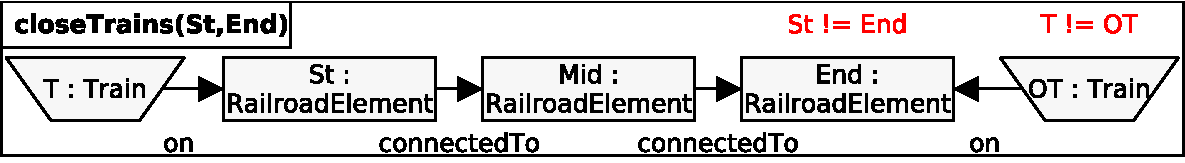
\includegraphics[width=0.75\textwidth]{figures/pattern-visual.pdf}
		\caption{Non-formal visual representation of a graph pattern}
		\label{pattern-visual}
	\end{center}
\end{figure}


\section{Local search}

Local search~\cite{bur-marton-msc} is an algorithm to provide matchings of a graph pattern in a graph. It is a depth-first search in the space of variable bindings. In the root of the search tree all the variables are unbound. Then with each constraint, we add a new level for the tree. The child of a variable binding is all the other variable binding where 
\begin{itemize}
	\item The bound variables of the parent are bound to the same values as the corresponding variable in the child
	\item The constraint is satisfied by the child
\end{itemize}

The search tree can be traversed without materializing it with depth-first search. This means, that the elements of the search tree are calculated on the fly, by modifying the parent variable binding.

To optimize the size of the search tree the order of the constraints must be chosen properly. 

\section{Distributed platform}

% adatok diszjunkt halmazokra bontva különböző csomópontra
% az algoritmusok is elosztottak, nem lesz összegyűjtve az infó, úgy van kiértékelve, hogy nincs aki mindent látna a rendszerből

As cyber-physical systems are distributed we must deal with the sensor data coming from different sensors at different computation units of the system. Sending the sensor data to one computation unit and evaluate on that cause different problems: Sensor data can be huge to send it through the network, the central node can be a SPOF, etc. In the presented framework the live model is distributed on the different computation units and the graph pattern matching algorithm itself runs in a distributed way. This eliminates the problem of central computers, but introduces complexity, that we must handle. 










%----------------------------------------------------------------------------
\chapter{Overview of the approach}
%----------------------------------------------------------------------------

%%
%% Futásidejű dolgok és kódgenerálás is!
%%


\begin{figure}[h]
	\begin{center}
		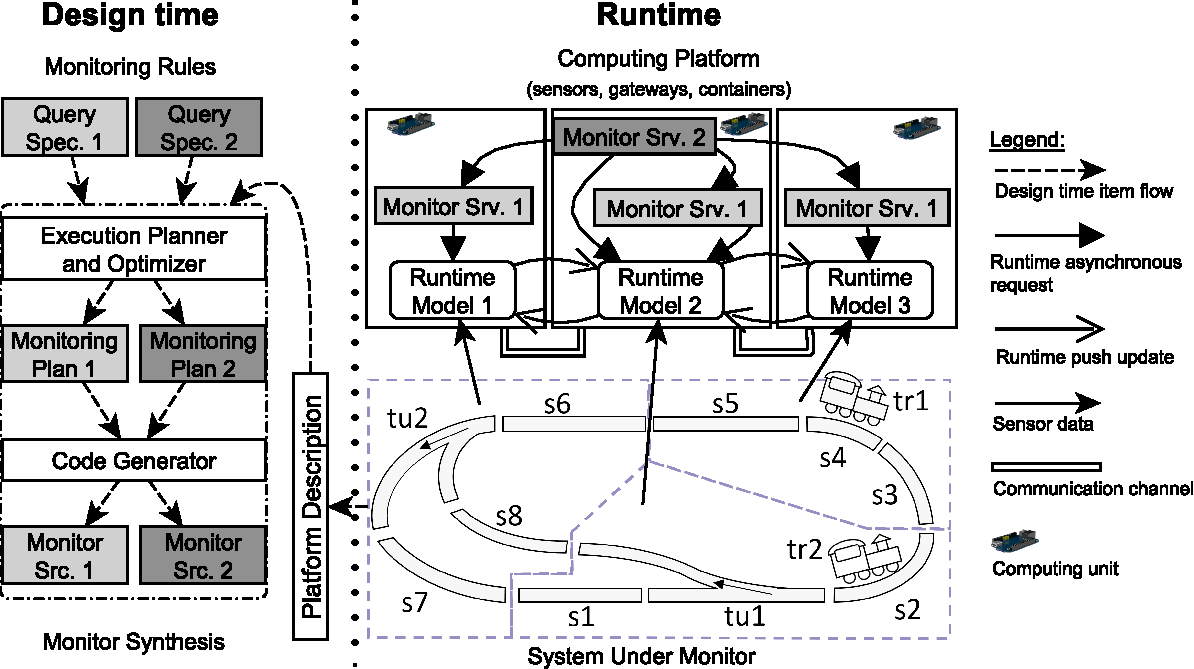
\includegraphics[width=\textwidth]{figures/fase-overview-crop.pdf}
	\end{center}
\end{figure}





%----------------------------------------------------------------------------
\chapter{Implementation details}
%----------------------------------------------------------------------------


\section{Overview of the query compilation workflow (batch approach, phases)}
\section{Localsearch planning}
\section{Supplementary TSystem}
\section{Additional optimization}
\section{C++ code generation}








%----------------------------------------------------------------------------
\chapter{Evaluation}
%----------------------------------------------------------------------------


\section{Measurement setup}

To measure the performance of the code generated by our framework we use the following setup. We use 6 BeagleBone Black (BBB) \cite{BBB} as computation units. We connect them via network. 

The model is partitioned to the units in 3 different ways 
\begin{itemize}
	\item Standard -- The model is partitioned by equally distributing the model considering locality ie.\ elements that are connected have more probability of being allocated to the same unit
	\item Alternative -- The model is partitioned by equally distributing the model not considering locality
	\item Single -- All of the elements are allocated on the same node
\end{itemize}

\section{Measurement result}








\section{Evaluation}

\chapter{Conclusions}
\label{sec:conclusion}

In this paper we introduced a novel runtime verification system for distributed CPS systems. The approach is based on the VIATRA-Query graph pattern language, which is used to define analysis properties. Graph models are used to define the structural information captured from the system. A code generator generates the data structures and the code to evaluate the queries on the model at runtime. The model is continuously updated with the information received from the environment and fast query execution provides runtime verification. 
The framework combines various technologies from the model-driven and also the CPS domain into a comprehensive approach. A case-study and measurements are used for evaluation purposes. 
The initial measurements show that the approach is capable of analyzing real life systems and the framework can provide fast results even running in microcomputers with low resources.

In the future we plan to continue this line of research. We hope to extend the model handling to provide more adaptability and new strategies have to be added to efficiently handle highly dynamic systems. In addition, we plan to extend the approach to handle temporal properties.
So there is much work left and there are several points where we can further improve the framework. 


Abstract
Introduction

Motivating example

Preliminaries

Architecture for runtime system

Implementation details (design time + runtime dolgok)

Evaluation






% Acknowledgements
%~~~~~~~~~~~~~~~~~~~~~~~~~~~~~~~~~~~~~~~~~~~~~~~~~~~~~~~~~~~~~~~~~~~~~~~~~~~~~~~~~~~~~~
%----------------------------------------------------------------------------
\chapter*{\koszonetnyilvanitas}\addcontentsline{toc}{chapter}{\koszonetnyilvanitas}
%----------------------------------------------------------------------------



% List of Figures, Tables
%~~~~~~~~~~~~~~~~~~~~~~~~~~~~~~~~~~~~~~~~~~~~~~~~~~~~~~~~~~~~~~~~~~~~~~~~~~~~~~~~~~~~~~
%\listoffigures\addcontentsline{toc}{chapter}{\listfigurename}
%\listoftables\addcontentsline{toc}{chapter}{\listtablename}


% Bibliography
%~~~~~~~~~~~~~~~~~~~~~~~~~~~~~~~~~~~~~~~~~~~~~~~~~~~~~~~~~~~~~~~~~~~~~~~~~~~~~~~~~~~~~~
\bibliography{bib/mybib}
\addcontentsline{toc}{chapter}{\bibname}


% Appendix
%~~~~~~~~~~~~~~~~~~~~~~~~~~~~~~~~~~~~~~~~~~~~~~~~~~~~~~~~~~~~~~~~~~~~~~~~~~~~~~~~~~~~~~
%----------------------------------------------------------------------------
\appendix
%----------------------------------------------------------------------------
\chapter*{\fuggelek}\addcontentsline{toc}{chapter}{\fuggelek}
\setcounter{chapter}{\appendixnumber}
%\setcounter{equation}{0} % a fofejezet-szamlalo az angol ABC 6. betuje (F) lesz
\numberwithin{equation}{section}
\numberwithin{figure}{section}
\numberwithin{lstlisting}{section}
%\numberwithin{tabular}{section}

%----------------------------------------------------------------------------
\section{Measured queries}
%----------------------------------------------------------------------------


\subsection{Benchmarked patterns}

\begin{lstlisting}[language = vql]
pattern trainLocations(train: Train, loc: RailRoadElement)
{
	Train.on(train, loc);
}
\end{lstlisting}

\begin{lstlisting}[language = vql]
pattern derailment(elem: RailRoadElement, train: Train)
{
	Turnout(turnout);
	RailRoadElement.train(elem,train);
	
	neg find connected(elem, turnout);
	find straightOrDivergent(turnout, elem);
}
\end{lstlisting}

\begin{lstlisting}[language = vql]
pattern CloseTrains(start : RailRoadElement, end : RailRoadElement)
{
	
	Train.on(t1,start);
	
	RailRoadElement.connectedTo(start,middle); // Has EOpposite, inverse navigation is effective even without model index
	RailRoadElement.connectedTo(middle, end);
	
	start != end; // This ensures that at least the start and end segment is different
	
	RailRoadElement.train(end, t2);
	
	t1 != t2; // A train may occupy two neighboring segments when moving; this is not a hazardous situation
	
	// Allocation-specific part of the query: global or local execution is based on the substitutions of c1 and c2
}
\end{lstlisting}

\begin{lstlisting}[language = vql]
pattern endOfSiding(train: Train, end: RailRoadElement, neighbor: RailRoadElement)
{
	RailRoadElement.connectedTo(end,neighbor);
	neg find otherNeighbor(end,neighbor,_);
	
	RailRoadElement.train(neighbor, train);	
}
\end{lstlisting}

\clearpage

\subsection{Helper patterns for benchmark patterns}


\begin{lstlisting}[language = vql]
private pattern connected(a : RailRoadElement, b : RailRoadElement){
	RailRoadElement.connectedTo(a,b);
}
\end{lstlisting}

\begin{lstlisting}[language = vql]
private pattern straightOrDivergent(turnout : Turnout, elem : RailRoadElement){
	Turnout.straight(turnout, elem);
} or {
	Turnout.divergent(turnout, elem);
}
\end{lstlisting}

\begin{lstlisting}[language = vql]
private pattern otherNeighbor(e : RailRoadElement, n1 : RailRoadElement, n2 : RailRoadElement){	
	RailRoadElement.connectedTo(e,n1);
	RailRoadElement.connectedTo(e,n2);
	n1 != n2;
}

\end{lstlisting}

\vfill

%----------------------------------------------------------------------------
%\clearpage\section{Measured queries}
%----------------------------------------------------------------------------



%\label{page:last}
\end{document}
